\documentclass[11pt]{article}

\usepackage[margin=1in]{geometry}
\usepackage{amsfonts, amsmath, amssymb}
\usepackage{fancyhdr, float, graphicx}
\usepackage[utf8]{inputenc} % Required for inputting international characters
\usepackage[T1]{fontenc} % Output font encoding for international characters
\usepackage{fouriernc} % Use the New Century Schoolbook font
\usepackage[nottoc, notlot, notlof]{tocbibind}
\usepackage{listings}
\usepackage{xcolor}
\usepackage{blindtext}
\usepackage{hyperref}
\hypersetup{
	colorlinks=true,
	linkcolor=black,
	filecolor=magenta,
	urlcolor=blue,
	pdfpagemode=FullScreen,
}

\definecolor{codegreen}{rgb}{0,0.6,0}
\definecolor{codegray}{rgb}{0.5,0.5,0.5}
\definecolor{codepurple}{rgb}{0.58,0,0.82}
\definecolor{backcolour}{rgb}{0.95,0.95,0.92}

\lstdefinestyle{mystyle}{
	backgroundcolor=\color{backcolour},
	commentstyle=\color{codegreen},
	keywordstyle=\color{magenta},
	numberstyle=\tiny\color{codegray},
	stringstyle=\color{codepurple},
	basicstyle=\ttfamily\footnotesize,
	breakatwhitespace=false,
	breaklines=true,
	captionpos=b,
	keepspaces=true,
	numbers=left,
	numbersep=5pt,
	showspaces=false,
	showstringspaces=false,
	showtabs=false,
	tabsize=2
}

\lstset{style=mystyle}

% Header and Footer
\pagestyle{fancy}
\fancyhead{}
\fancyfoot{}
\fancyhead[L]{\textit{\Large{Blockchain Technology}}}
\fancyhead[R]{\textit{Krishnaraj T}}
\fancyfoot[C]{\thepage}
\renewcommand{\footrulewidth}{1pt}

\begin{document}

\begin{titlepage}
	\centering

	%---------------------------NAMES-------------------------------

	\huge\textsc{
		MIT World Peace University
	}\\

	\vspace{0.75\baselineskip} % space after Uni Name

	\LARGE{
		Attack Research and Documentation\\
		Fourth Year B. Tech, Semester 8
	}

	\vfill % space after Sub Name

	%--------------------------TITLE-------------------------------

	\rule{\textwidth}{1.6pt}\vspace*{-\baselineskip}\vspace*{2pt}
	\rule{\textwidth}{0.6pt}
	\vspace{0.75\baselineskip} % Whitespace above the title

	\huge{\textsc{
        To understand and Simulate Blockchain using Online Simulator
        }} \\

	\vspace{0.5\baselineskip} % Whitespace below the title
	\rule{\textwidth}{0.6pt}\vspace*{-\baselineskip}\vspace*{2.8pt}
	\rule{\textwidth}{1.6pt}

	\vspace{1\baselineskip} % Whitespace after the title block

	%--------------------------SUBTITLE --------------------------	

	\LARGE\textsc{
		Lab Assignment 1
	} % Subtitle or further description
	\vfill

	%--------------------------AUTHOR-------------------------------

	Prepared By \vspace{0.5\baselineskip} % Whitespace before the editors

	\Large{
		Krishnaraj Thadesar \\
		Cyber Security and Forensics\\
        Batch A1, PA 15
	}

	\vspace{0.5\baselineskip} % Whitespace below the editor list
	\today

\end{titlepage}

\tableofcontents
\thispagestyle{empty}
\clearpage

\setcounter{page}{1}

\section{Aim}
To understand and simulate Blockchain using an online simulator.


\section{Simulation}

\begin{figure}[H]
    \centering
    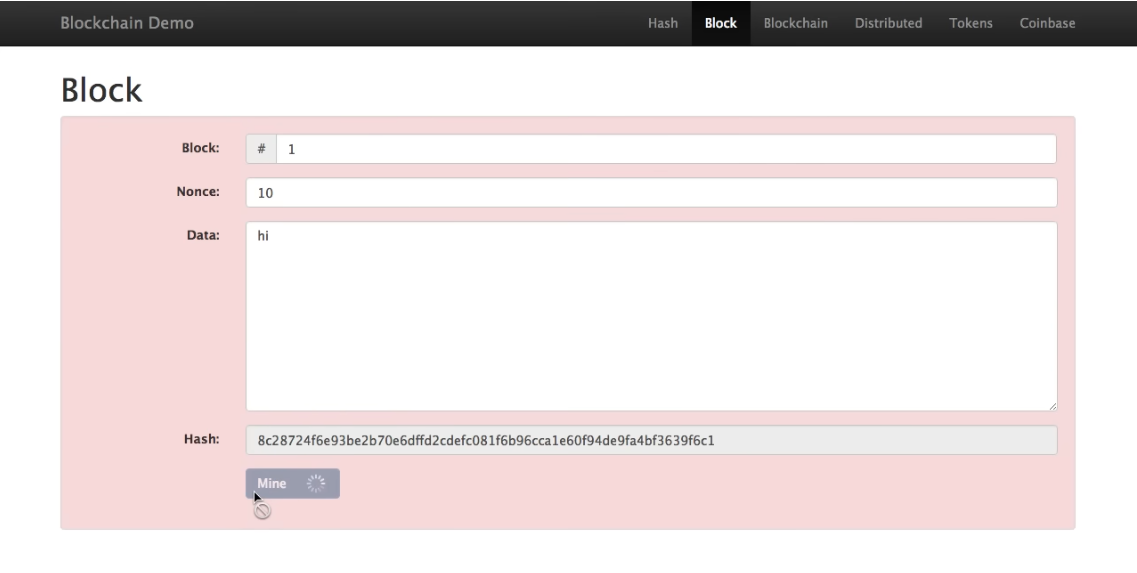
\includegraphics[width=0.8\textwidth]{1.png}
    \caption{A Block}
    \label{fig:1}
\end{figure}

\begin{figure}[H]
    \centering
    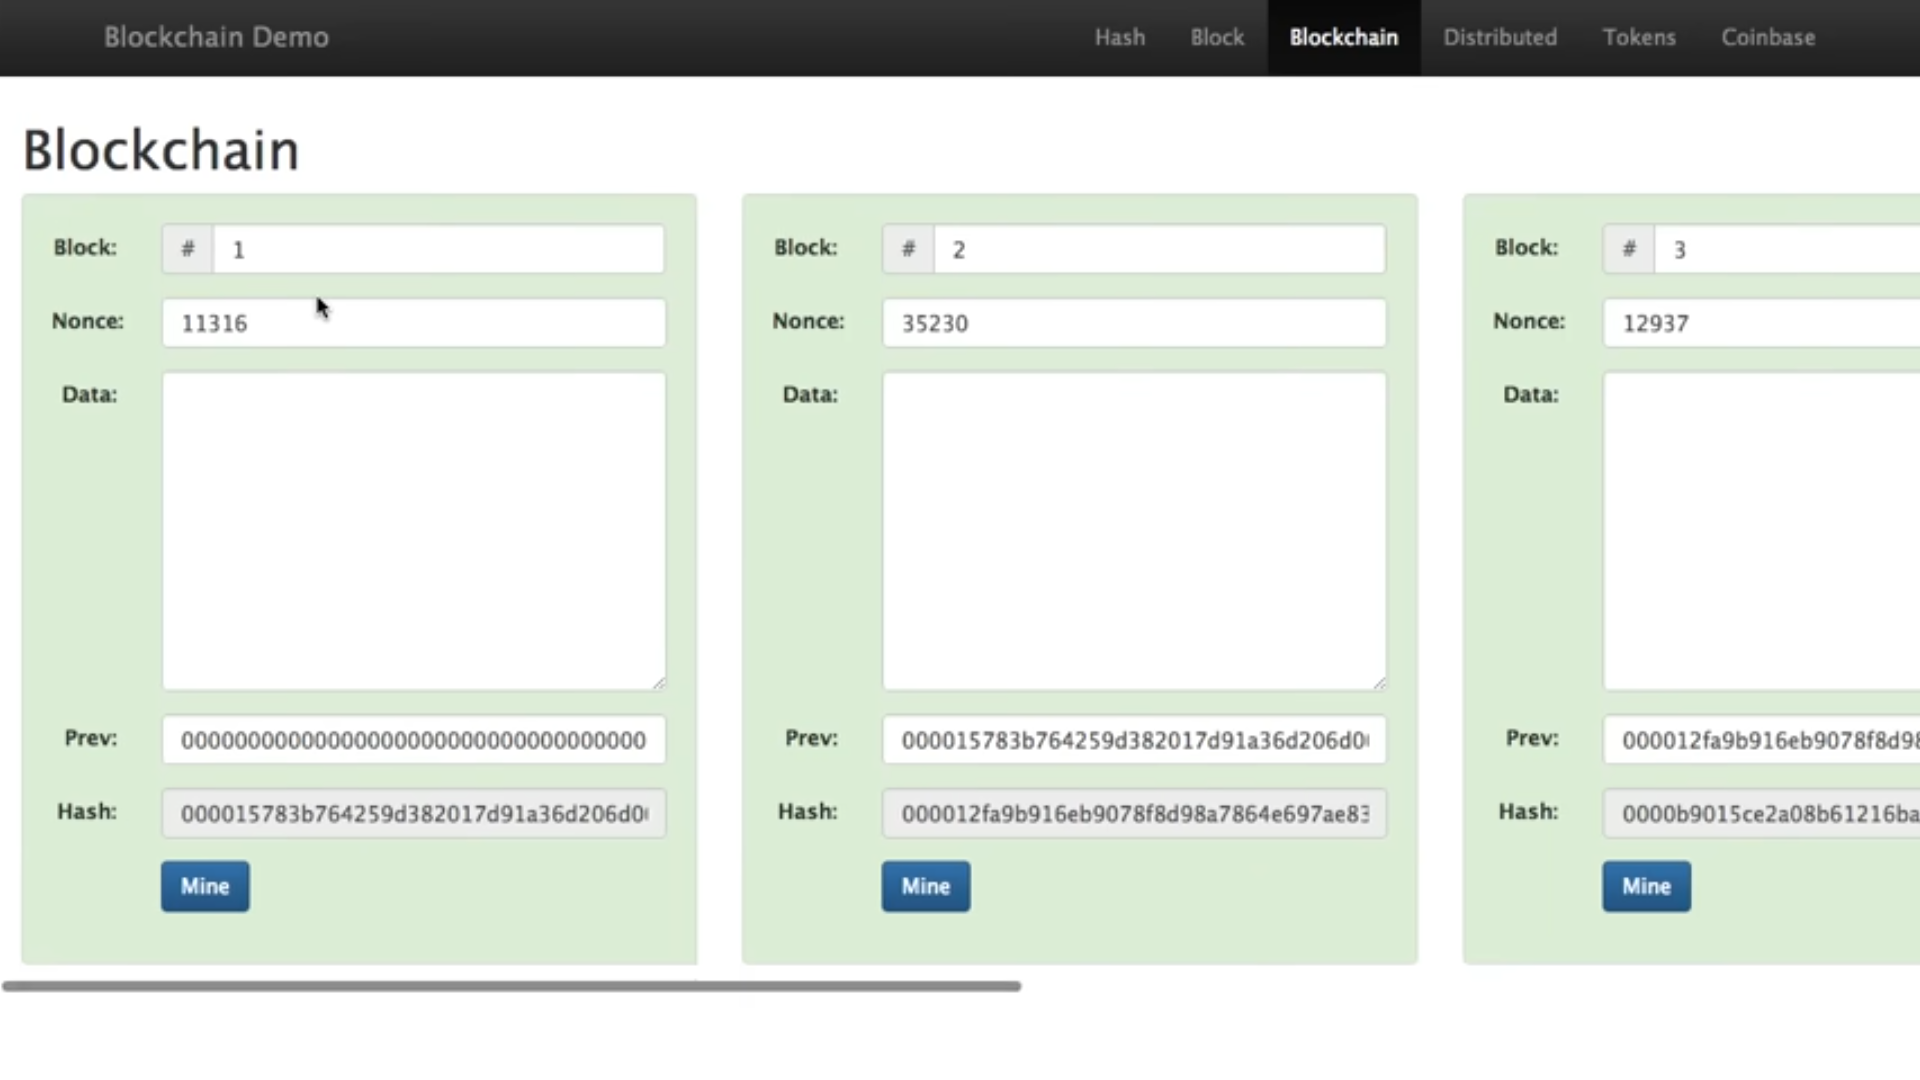
\includegraphics[width=0.8\textwidth]{2.png}
    \caption{Some Blocks forming a chain}
    \label{fig:1}
\end{figure}

\begin{figure}[H]
    \centering
    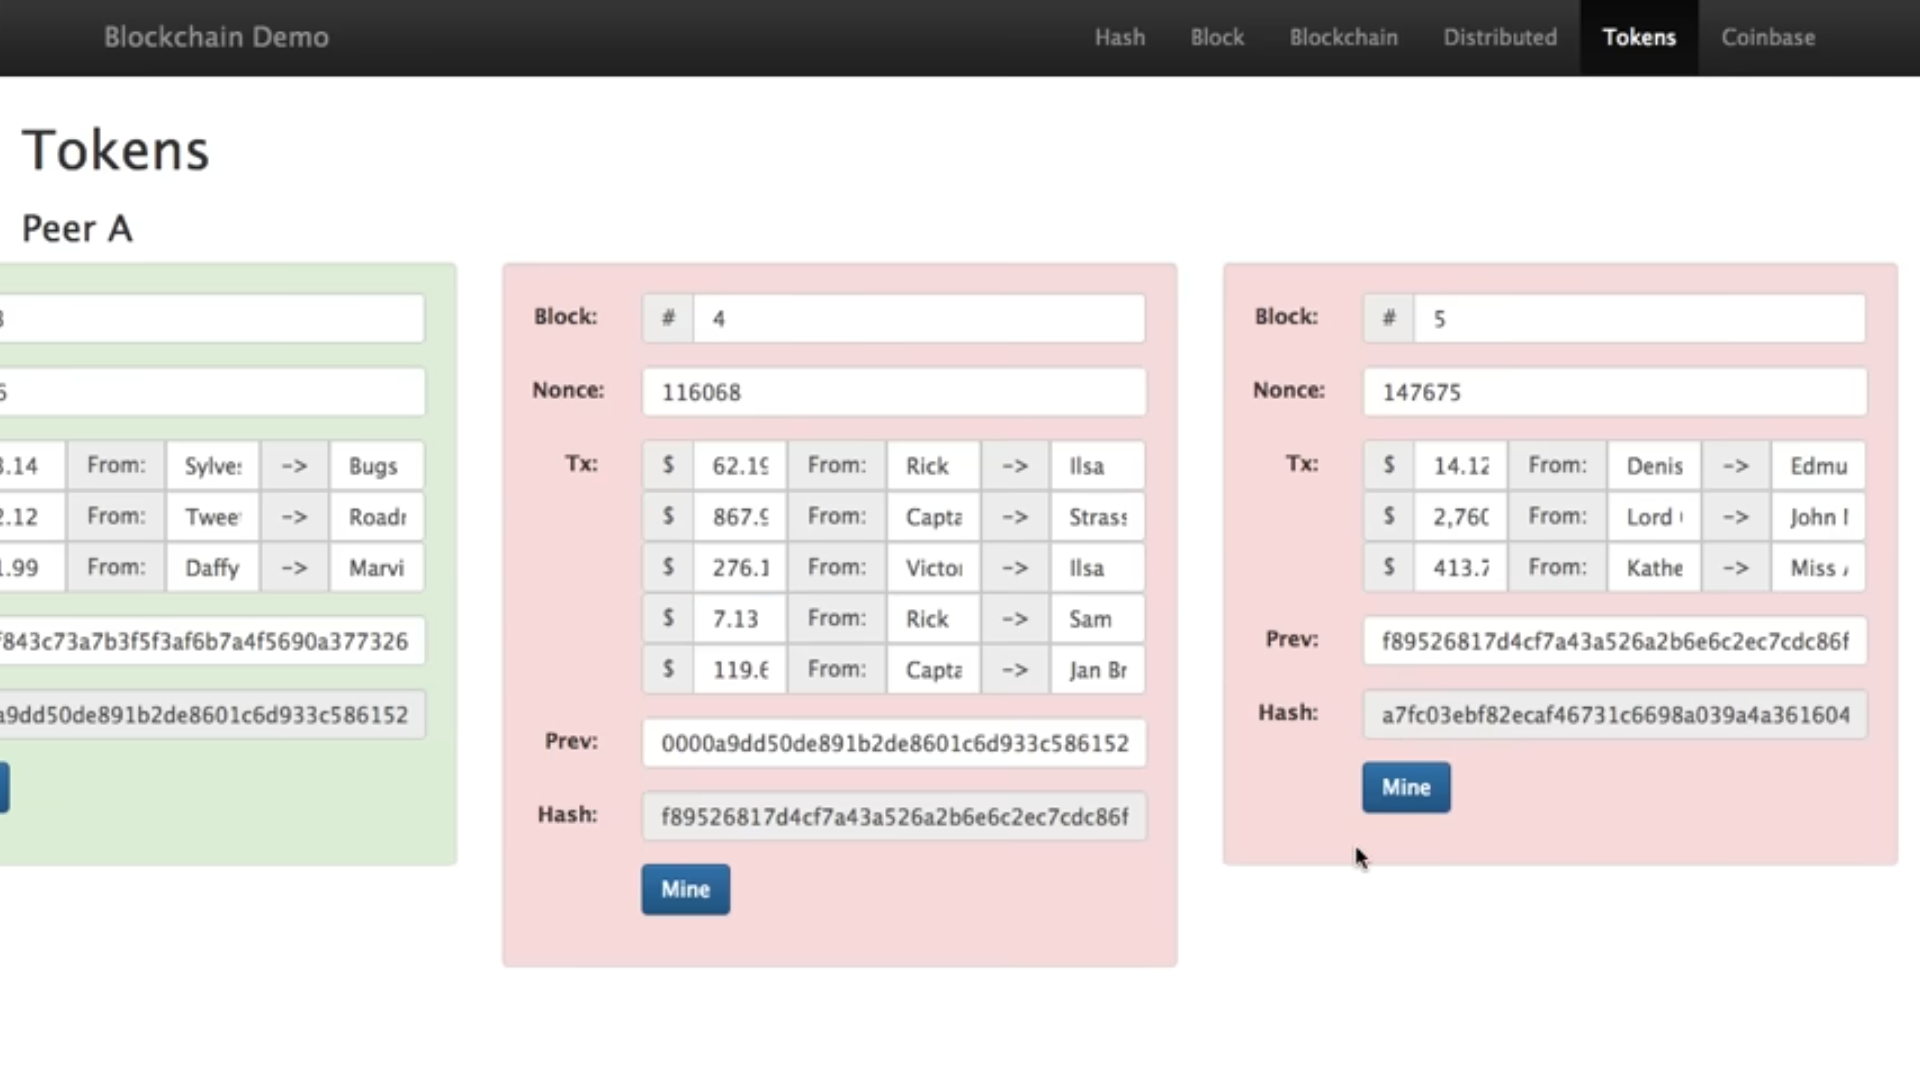
\includegraphics[width=0.8\textwidth]{3.png}
    \caption{Tokens}
    \label{fig:1}
\end{figure}

\section{Frequently Asked Questions}

\subsection{What is blockchain technology and how does it differ from traditional databases?}

Blockchain is a decentralized and distributed ledger technology that records transactions across multiple nodes securely and immutably. Unlike traditional databases, which are typically centralized and controlled by a single entity, blockchain operates in a peer-to-peer network, making it more secure and tamper-resistant. Data in blockchain is stored in linked blocks rather than tables and rows, ensuring transparency and integrity.

\subsection{Who invented Blockchain? What was its original purpose?}

Blockchain was introduced in 2008 by an anonymous person or group under the pseudonym \textit{Satoshi Nakamoto}. It was originally designed as the underlying technology for Bitcoin, enabling a decentralized and trustless digital currency system without the need for a central authority.

\subsection{How does a decentralized network work in blockchain and why is it important?}

A decentralized network in blockchain consists of multiple nodes (computers) that validate and store transactions. Each node maintains a copy of the blockchain, and consensus mechanisms (e.g., Proof of Work or Proof of Stake) ensure agreement on the ledger’s state. Decentralization enhances security, prevents a single point of failure, and reduces reliance on intermediaries.

\subsection{What is a 'Block' in a blockchain? How does it store data?}

A block in a blockchain is a digital container that stores transaction data, a timestamp, a reference to the previous block (hash), and a cryptographic proof (such as a nonce). Transactions within a block are hashed and linked together, ensuring integrity and immutability. Each new block is appended to the chain sequentially, forming a continuous and verifiable record.

\subsection{How does a transaction get verified and added to a blockchain?}

Transactions are verified through a consensus mechanism. In Proof of Work (PoW), miners solve complex mathematical puzzles to validate transactions and create new blocks. In Proof of Stake (PoS), validators are chosen based on the amount of cryptocurrency they hold. Once verified, a transaction is added to a block, and the block is appended to the blockchain after network consensus.

\subsection{What is the role of cryptography in ensuring the security and integrity of a blockchain?}

Cryptography plays a crucial role in blockchain security by ensuring data confidentiality, integrity, and authentication. Hash functions (e.g., SHA-256) generate unique digital fingerprints for blocks, making them tamper-proof. Public-key cryptography enables secure transactions by allowing users to sign and verify data using private and public keys.

\subsection{What are the key benefits of blockchain for industries like finance, supply chain, and healthcare?}

\begin{itemize}
    \item \textbf{Finance:} Enables secure, fast, and transparent transactions, reducing fraud and eliminating intermediaries.
    \item \textbf{Supply Chain:} Enhances traceability, prevents counterfeit products, and improves efficiency in tracking goods.
    \item \textbf{Healthcare:} Ensures secure patient records, facilitates interoperability, and protects sensitive medical data.
\end{itemize}

\subsection{What challenges does blockchain face in terms of scalability, energy consumption, and regulatory concerns?}

\begin{itemize}
    \item \textbf{Scalability:} Blockchain networks, especially those using PoW, have limited transaction throughput compared to traditional systems.
    \item \textbf{Energy Consumption:} Mining in PoW-based blockchains consumes vast amounts of energy, raising environmental concerns.
    \item \textbf{Regulatory Concerns:} Many governments struggle with regulatory frameworks due to the decentralized and pseudonymous nature of blockchain transactions.
\end{itemize}

\subsection{How does blockchain promote transparency and trust in digital transactions?}

Blockchain promotes transparency by making all transactions publicly verifiable while ensuring data integrity. Since transactions are immutable and time-stamped, users can trust the authenticity of the recorded data without relying on central authorities.

\subsection{What are some real-world examples of how blockchain technology is being used today?}

\begin{itemize}
    \item \textbf{Cryptocurrencies:} Bitcoin, Ethereum, and other digital currencies operate on blockchain networks.
    \item \textbf{Smart Contracts:} Ethereum enables automated, self-executing contracts without intermediaries.
    \item \textbf{Supply Chain Management:} IBM's Food Trust blockchain enhances food safety and traceability.
    \item \textbf{Healthcare:} Estonia uses blockchain to secure medical records and ensure data privacy.
    \item \textbf{Voting Systems:} Some governments experiment with blockchain-based voting to enhance election security.
\end{itemize}

\section{Conclusion}

Blockchain technology is a revolutionary advancement that enhances security, transparency, and decentralization across various industries. While it faces challenges such as scalability and regulatory concerns, continuous innovation is leading to more efficient solutions. As adoption grows, blockchain has the potential to redefine digital transactions and trust mechanisms in the modern world.


% \begin{figure}[H]
%     \centering
%     \includegraphics[width=0.8\textwidth]{}
%     \caption{}
%     \label{fig:1}
% \end{figure}

\clearpage
\begin{thebibliography}{99}

\bibitem{nakamoto2008bitcoin}
Nakamoto, S. (2008). Bitcoin: A Peer-to-Peer Electronic Cash System. Retrieved from \url{https://bitcoin.org/bitcoin.pdf}

\bibitem{wood2014ethereum}
Wood, G. (2014). Ethereum: A Secure Decentralised Generalised Transaction Ledger. Ethereum Project Yellow Paper, 151, 1-32.

\bibitem{pilkington2016blockchain}
Pilkington, M. (2016). Blockchain technology: principles and applications. In Research Handbook on Digital Transformations (pp. 225-253). Edward Elgar Publishing.

\bibitem{rosenfeld2011analysis}
Rosenfeld, M. (2011). Analysis of hashrate-based double spending. arXiv preprint arXiv:1402.2009.

\bibitem{swanson2015consensus}
Swanson, T. (2015). Consensus-as-a-service: a brief report on the emergence of permissioned, distributed ledger systems. Report, available at \url{http://www.ofnumbers.com/wp-content/uploads/2015/04/Permissioned-distributed-ledgers.pdf}

\end{thebibliography}

\end{document}